\documentclass[12pt]{article}

\usepackage{times}
\usepackage{amsmath}
\usepackage{latexsym}
\usepackage{fullpage}
\usepackage{graphicx}
\usepackage{amsfonts}

\graphicspath{ {./images/} }

\newcommand{\NOT}{\neg}
\newcommand{\AND}{\wedge}
\newcommand{\OR}{\vee}
\newcommand{\XOR}{\oplus}
\newcommand{\IMPLIES}{\rightarrow}
\newcommand{\IFF}{\leftrightarrow}
\newcommand{\E}{\exists}
\newcommand{\A}{\forall}

\setlength{\parskip}{.1in}

\renewcommand{\baselinestretch}{1.1}

\begin{document}

\begin{center}

{\bf
CSCE 313\\
PA5-Report\\
Jeffrey Xu\\
11/06/20\\
}

\end{center}

\section{Runtime Analysis}

We want to analyze the runtime of our program when we vary different variables. For this report, we will follow similar formats as was in PA4 and vary the $b$ and $w$ parameters. For $b$, we will test values from $[1,200]$ and for $w$, we will test values in the range $[1,500]$. We will use $n=15000$ and $p=15$ when performing our tests. We will also hold $w=500$ and $b=100$ when testing. The graph plots are shown below. 

\begin{center}
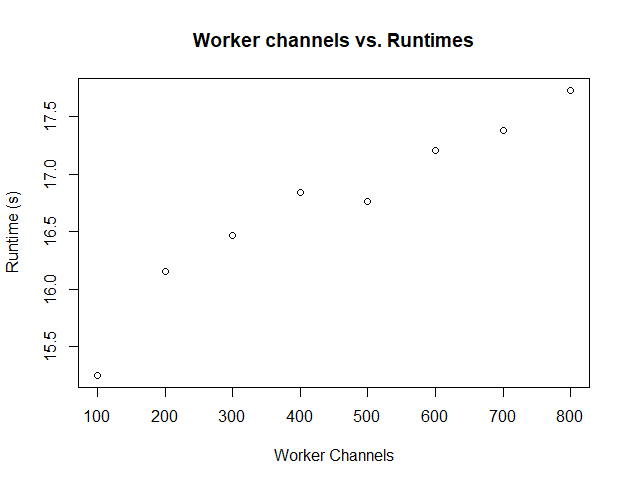
\includegraphics[width=8cm, height=6cm]{w_vs_run}
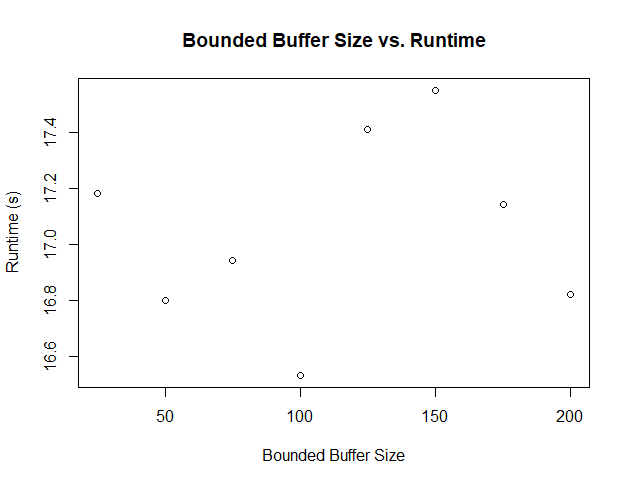
\includegraphics[width=8cm, height=6cm]{b_vs_run}
\end{center}

We notice a completely opposite trend here with the worker channels. This may be because of how we are only using one thread that uses $w$ worker channels. Since it is only one thread, it still basically has to run each request sequentially. Therefore, having more worker channels may not always give a better runtime. We notice a diminishing point for the worker channels at around $w=500$ which was about the same point for PA4. 

For the bounded buffer, we don't really see any trend with the bounded buffer size versus the runtime. We noticed this trend as well with PA4 since the size of the bounded buffer won't really make a difference in performance. This is mainly because the capacity of the bounded buffer doesn't determine the speed at which our threads or channels execute each request in this case. 

The shape of the bounded buffer graph is around the same with PA4, but the graph for the worker channels is basically an inverse of what the worker thread graph was in PA4. This is probably because we only have one thread for the workers and we are basically running the worker threads sequentially since there is only one thread. Therefore, having more worker channels could result in more overhead as our code needs to handle more channels and make sure they all work in order. This is completely different compared to PA4 when we basically had each channel working in parallel which resulted in the runtime decrease as we had more worker threads since more are running in parallel. 

Video Link: https://youtu.be/pKjqN3NfQBY

\end{document}